\section{Proposed World Model and System Architecture}
\label{sec:architecture}

This section shall focus in suggestion in world model contruction, the whole agent interaction flow, and training algorithm that shall be leveraged

\subsection{Notation}
Our problem can be formalizing as the deterministic Markov Decision Process (MDP) with the usage of internal continuous stochastic states and derterministic state, and yeilding the deterministic continuous action in the finite-horizontal enviroment as \cite{sun_2022_supervised, Hafner2023} suggested. The MDP can be defined as the tuples in Eq.~\eqref{eq:MDP}

\begin{equation}
\label{eq:MDP}
\mathcal{M} = (\mathcal{S}, \mathcal{A}, \mathcal{P}, r, \gamma),
\end{equation}

where $\mathcal{S}$ denotes the (possibly continuous) state space, 
$\mathcal{A}$ denotes the (possibly continuous) action space, 
$\mathcal{P}(s_{t+1} \mid s_t, a_t)$ represents the state transition dynamics which including the stochastic states $s_t$ capturing the enviroment randomness pattern within the transition, and determistic states $h_t$ yeild from the recurrent-planner for historical context,
$r : \mathcal{S} \times \mathcal{A} \rightarrow \mathbb{R}$ is the reward function,
and $\gamma \in [0,1)$ is the discount factor - and for the setting we are adopt dirrectly the setting of DreamerV3 by setting  $\gamma$ = 0.997.

The action space we attempts including the ego's vehicle acceleration, and steering angle (in radian) as the response for making the interaction to the simmulation.

\subsection{Overall System Architecture}
The proposed overall system archtiecture include modules as enviroment interface, which build based on the HighwayEnv package provided by \cite{faramafoundation_2025_gymnasium} for agent interaction, we additionally including the Transtion Queues with limited in size as the experience collector for the World Model can be sampling randomly certain episode from the queue that have with satisfied sequence length $T$, the World Model shall provide the imaginary embedding as the train-signal toward the Actor-Critic controler head for yielding the action for reacting toward the enviroment and create an close interacting cycle until the agent reach the terminatin states, the architecture of the whole HanoiWorld is presented on the right side of Figure~\ref{fig:architecture_and_world_model}.
    
The transition queue shall storing the list of episode (eg. reference of valid episode) that have the length of transition satisfy certain threadshold - $T$, and the sequence shall contain the Bird-Eye-View RGB images and the metadata on the agent's interaction as the agent's action, ego's actions, and the description on the reward been yield across the simulation for those sequence.

\begin{figure}[t]
    \centering
    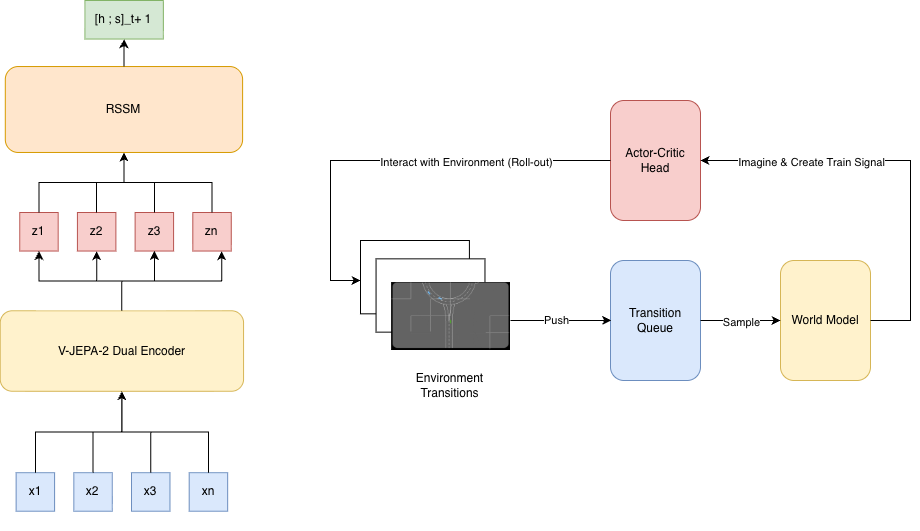
\includegraphics[width=0.85\linewidth]{Figure/HanoiWorld_Agent.png}
    \caption{The proposed HanoiWorld World Model (left) include an visual encoder based on V-JEPA-2 checkpoint proposed by \cite{assran_2025_vjepa} and the RSSM-backbone suggested by \cite{hafner_2019_learning} for making long-term planning on the next possible transition of enviroment - the green block. The overal system arrchitectural of the enviroment on the (right) which been design aiming for both effective rolling-out while model training from the enviroment by creating such feedback loop on the agent interaction with data-scarcity}
    \label{fig:architecture_and_world_model}
\end{figure}

\subsection{HanoiWorld - The World Model}

\subsubsection*{V-JEPA 2 Based Encoder}

The main innovation of the HanoiWorld is the inclusion of the strong pretrained image encoder based on self-supervised learning manner proposed by \cite{assran_2025_vjepa}. Specifically, the V-JEPA 2 aim at learning the essential knowledge on enviroment interaction as the motion, object movement , without focusing on the stochasitic and noisy pixel detail as reconstruction attemps as DreamerV3-based encoders \cite{Hafner2023, hu_2023_gaia1}. The V-JEPA 2 encoder shall be trained to predict the masked version of the corresponding input follow self-supervising manner for more 1 million hours of video, and be stablized using Exponential Moving Average (EMA) in the Student-Teacher scheme for preventing the embedding collaspe while maintaining essential feature are strucutrally preserved \cite{caron_2021_emerging}.

\begin{figure}[t]
    \centering
    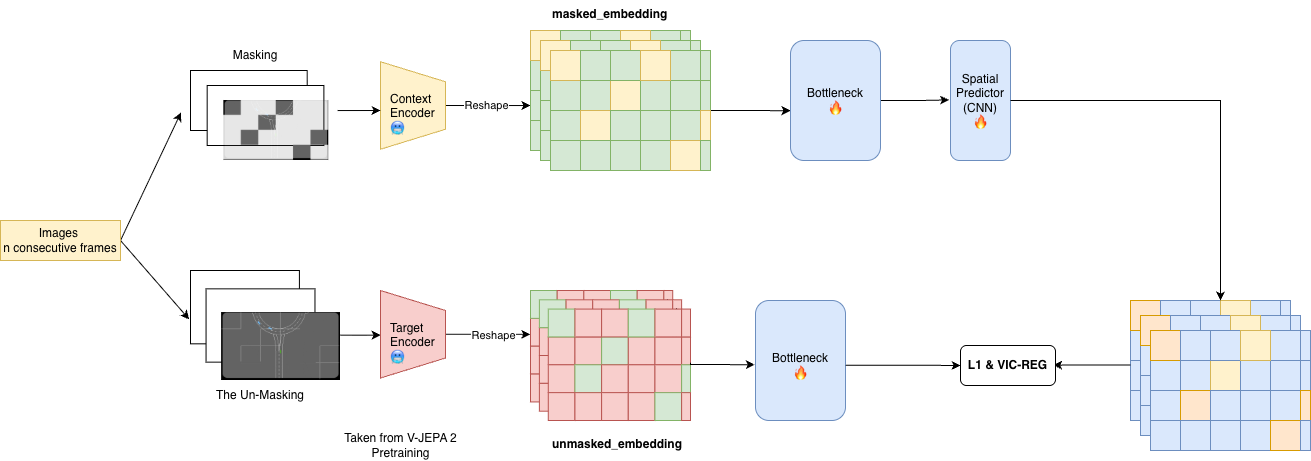
\includegraphics[width=0.85\linewidth]{Figure/Encoder_Archi.png}
    \caption{Overview of the proposed HanoiWorld encoder architecture.
    A pretrained and frozen V-JEPA~2 encoder~\cite{assran_2025_vjepa} is used as a high-quality representation backbone to improve training efficiency and embedding robustness under limited-data settings.
    A downstream bottleneck Multi-Layer Perceptron (MLP) is trained to project the high-dimensional representations into a compact and task-compatible latent space of size $1024 \times 128$.
    In parallel, the student encoder branch incorporates an additional 2D convolutional neural network (CNN) module to predict spatial representations.
    Both branches are jointly optimized using an $\ell_1$ alignment loss as Eq.~\eqref{eq:jepa_loss} and the VICReg regularization objective~\cite{bardes_2022_vicreg}.}
    \label{fig:encoder_architecture}
\end{figure}

\paragraph{EMA Teacher Encoder.}
Let $\theta$ denote the parameters of the student encoder $E_\theta$
and $\bar{\theta}$ denote the parameters of the teacher encoder.
The teacher parameters are updated using an exponential moving average:
\begin{equation}
\bar{\theta}
\;\leftarrow\;
\tau\,\bar{\theta}
+
(1 - \tau)\,\theta,
\label{eq:ema_update}
\end{equation}
where $\tau \in [0,1)$ is the momentum coefficient.
Gradients are stopped through the teacher encoder to prevent representation collapse, and in our experiment, we set $\tau$ = 0.996.


\paragraph{Masked Representation Prediction.}
Given a video $y$ and a masked view $x$ obtained by removing a subset of spatio-temporal patches,
the encoder $E_\theta$ extracts representations from the visible tokens.
A predictor $P_\phi$ is trained to predict the representations of the masked tokens.

The main training objective is defined as the L1-Loss as the Eq.~\eqref{eq:jepa_loss}:

\begin{equation}
\mathcal{L}_{\text{align}}
=
\left\|
P_\phi\!\left(\Delta_y, E_\theta(x)\right)
-
\operatorname{sg}\!\left(E_{\bar{\theta}}(y)\right)
\right\|_1,
\label{eq:jepa_loss}
\end{equation}

where $\Delta_y$ denotes learnable mask tokens indicating the locations of the masked patches,
and $\operatorname{sg}(\cdot)$ denotes the stop-gradient operator.
The loss is applied only to the masked patches, and we leverage the patch-mask with random-masking as \cite{mo_2024_connecting} suggest for the finetuning process.

The leverage of the dual-branch self-supervised training with masking pattern does occur in work of \cite{zhu_2025_selfsupervised}, in which suggest that by let the encoder have to force to guess the masked patch from the sampel - which does creating challenge for preventing embedding collaspe while occupancy semenatic can be learn and predicted without the need of full geometrical structure on the enviroment.

\subsubsection*{RSSM-Based Reasoning Model}

The RSSM (Recurrent State-Space Model) our design is follow the codebase provided with the DreamerV3 architecture by \cite{hafner_2019_learning, Hafner2023}, the purpose of RSSM considered as the internal-memory module that storing the deterministic memory for long-term historical semantics, and the stochastic latent values as the uncertainty prediction based on the enviroment encoded-signals for capturing the world's evolution, and agent's expected prior conditioned by the world's state transformation. The generative process on yeilding the World Dynamics can be formulated as the follow Eq.~\eqref{eq:rssm_generative}

\begin{equation}
\label{eq:rssm_generative}
\begin{aligned}
h_t &= f_\theta(h_{t-1}, z_{t-1}, a_{t-1}), \\
z_t &\sim p_\theta(s_t \mid h_t), \\
z_t &\sim p_\theta(z_t \mid h_t, z_t), \\
r_t &\sim p_\theta(r_t \mid h_t, z_t).
\end{aligned}
\end{equation}

Given that:
\begin{itemize}
    \item $f_\theta$ denotes the recurrent dynamics function parameterized by $\theta$,
    implemented as a recurrent neural network.
    \item $h_t$ represents the deterministic latent state at time step $t$.
    \item $a_t$ denotes the action executed by the agent at time step $t$.
    \item $z_t$ corresponds to the observation at time step $t$, which in our setting
    is the V-JEPA-2 encoded embedding for the corresponding time step.
    \item $r_t$ denotes the predicted reward yielded by the agent at time step $t$.
    \item All conditional distributions $p_\theta(\cdot)$ are parameterized by
    multi-layer perceptron (MLP) decoder networks.
\end{itemize}

Additionally, as the HanoiWorld migrating the RSSM-codebased from the DreamerV3, the model does additional including a continue-predictor for guessing whether the episode shall be continue given the encoder embedding $o_t$, and historical latent images $z_t$ \cite{Hafner2023} - showcased with Eq.~\eqref{eq:continue_predictor}, given the continuation signal is a Bernouli random variable for simplified assumption.

\begin{equation}
\label{eq:continue_predictor}
c_t \sim p_\theta(c_t \mid h_t, z_t),
\end{equation}
where $c_t \in \{0,1\}$ indicates whether the episode continues at time step $t$.

The continue-predictor training as the logistic-regression model using the binary-cross-entropy as the original DreamerV3 suggestion with the Eq.~\eqref{eq:continuation_loss}
\begin{equation}
\label{eq:continuation_loss}
\mathcal{L}_{\text{cont}}
=
-
\left[
c_t \log \hat{c}_t
+
(1 - c_t)\log(1 - \hat{c}_t)
\right].
\end{equation}

\begin{itemize}
    \item $c_t \in \{0,1\}$ denotes the ground-truth binary continuation label at time step $t$.
    \item $\hat{c}_t \in (0,1)$ denotes the predicted continuation probability produced by the model.
\end{itemize}

\subsection{The Actor-Critic Training Head}

The HanoiWorld Actor--Critic framework is directly derived from the reward- and value-based learning paradigm of DreamerV3. It shares core conceptual foundations with the classical theory proposed by \cite{sutton_1991_dyna}, which emphasizes a separation between an \emph{Actor} network (policy network) that reacts by selecting actions and a \emph{Critic} network that evaluates the agent's performance through a value function in order to support more effective planning. However, unlike the classical Actor--Critic formulation in \cite{sutton_1991_dyna}, which operates on actual environment states, the DreamerV3 Actor--Critic operates entirely in a learned latent environment. Specifically, both the policy network $\pi_\theta$ and the value network $v_\psi$ are defined over the latent state $\ell_t$ produced by the RSSM, as formalized in Eq.~\eqref{eq:actor_critic_latent}.

\begin{equation}
\label{eq:actor_critic_latent}
\ell_t = (h_t, z_t), \qquad
a_t \sim \pi_\theta(a_t \mid \ell_t), \qquad
v_\psi(R_t \mid \ell_t).
\end{equation}

Given that:
\begin{equation}
R_t = \sum_{k=0}^{\infty} \gamma^k r_{t+k}.
\end{equation}

\begin{itemize}
    \item $\ell_t = (h_t, z_t)$ denotes the latent state at time step $t$,
    consisting of the deterministic and stochastic components of the RSSM and V-JEPA-2 encoder respectively.
    \item $R_t$ denotes the return at time step $t$, defined as the discounted
    sum of future rewards over an episode,
    with discount factor $\gamma = 0.997$.
\end{itemize}

\subsection{Training Procerdure an Objective }

HanoiWorld training objective including the Spatial Predictor and Predictor training in the Encoder module, and training the RSSM-dynamics based model, with the Actor-Critic training follow. Given that HanoiWorld training tactics only mimicking the training procedure of DreamerV3 on the Dynamics, and Actor-Critic network, not the reconstructed-based training for encoder as \cite{Hafner2023}.

\subsubsection*{Encoder Training}

For the Bottleneck and Spatial Predictor training, beside using the L1-loss as Eq.~\eqref{eq:jepa_loss}, we consider the usage of Variance Correlation and Covariance Regularization suggested by \cite{bardes_2022_vicreg} - check Eq.~\eqref{eq:var} and Eq.~\eqref{eq:covar}

\begin{equation}
\label{eq:var}
\mathcal{L}_{\text{var}}
=
\frac{1}{D}
\sum_{d=1}^{D}
\max\!\left(0,\;
1 - \sqrt{\operatorname{Var}\!\left(\tilde{z}_{:,d}\right) + \varepsilon}
\right),
\end{equation}

\begin{equation}
\label{eq:covar}
\mathcal{L}_{\text{cov}}
=
\frac{1}{D}
\sum_{i \neq j}
\left(
\operatorname{Cov}(\tilde{z})_{ij}
\right)^2,
\end{equation}

\begin{equation}
\label{eq:covar_mat}
\operatorname{Cov}(\tilde{z})
=
\frac{1}{BN - 1}
\left(
\tilde{\mathbf{z}} - \bar{\mathbf{z}}
\right)^{\!\top}
\left(
\tilde{\mathbf{z}} - \bar{\mathbf{z}}
\right),
\end{equation}

Given that:

\begin{itemize}
    \item $D$ denotes the embedding dimensionality (D=128), and
    $\tilde{\mathbf{z}} \in \mathbb{R}^{(BN)\times D}$ represents the flattened
    embeddings obtained by reshaping the batch and token dimensions.
    \item $\tilde{z}_{:,d}$ refers to the $d$-th embedding dimension across
    all $BN$ samples, and $\varepsilon$ is a small constant added for numerical
    stability.
    \item The variance regularization in Eq.~\eqref{eq:var} enforces a minimum
    standard deviation for each embedding dimension, preventing representational
    collapse.
    \item $\epsilon$ standfor the small constant for numerical stability as $\epsilon$ = 1e-4
    
    \item The covariance matrix $\operatorname{Cov}(\tilde{z})$ in
    Eq.~\eqref{eq:covar_mat} is computed after centering the embeddings by their
    mean $\bar{\mathbf{z}} = \frac{1}{BN}\sum_{i=1}^{BN}\tilde{\mathbf{z}}_i$.
    \item The covariance regularization in Eq.~\eqref{eq:covar} penalizes the
    squared off-diagonal entries of the covariance matrix, encouraging
    decorrelation between different embedding dimensions.
\end{itemize}

The Bottleneck are train that follow the weighted sum loss function as follow \cite{bardes_2022_vicreg, assran_2025_vjepa, zhu_2025_selfsupervised}, and with the weights are setup toward  ($\alpha$, $\beta$, $\gamma$) to (1.0, 1.0, 0.1) for stability and prevent collaspe, and lossely controlling the covariance between teacher's bottleneck and student's predictor.

\begin{equation}
\mathcal{L}_{\text{encoder}}
=
\alpha\,\mathcal{L}_{\text{align}}
+
\beta\,\mathcal{L}_{\text{var}}
+
\gamma\,\mathcal{L}_{\text{cov}}.
\end{equation}

We does finetune our encoder on the 2D Bird-Eye-View dataset which have been pre-processed from the Nuscene dataset proposed by \cite{Caesar2021} by rendering from the LiDAR-cloud based with additional metadata on the obstacle and enviroment movement toward the RGB based images that V-JEPA 2 encoder can working with.

\subsubsection*{RSSM-dynamic model training}

For the RSSM module training, we leverage the usage of predictor loss which is the inverse summation on the log probability of the probability in guessing the actual observation on the enviroment's transition, the reward function, and continue flag as Eq~\eqref{eq:L_pred}; the dynamicity loss by minimalizing the KL-diveregnce between actual posterior distribution encoder yeild out from actual observation stably, with prior that world model imagine from prior-latent memory as Eq~\eqref{eq:L_dyn}; and the representation loss for anchoring the encoder without drifting away from latent world model expectation in Eq~\eqref{eq:L_rep}. This loss-setup follows the work of \cite{Hafner2023} suggested and using the identical weight-set as DreamerV3 been configured before.

\begin{align}
\mathcal{L}_{\text{pred}}(\phi)
&=
- \log p_\phi(x_t \mid z_t, h_t)
- \log p_\phi(r_t \mid z_t, h_t)
- \log p_\phi(c_t \mid z_t, h_t),
\label{eq:L_pred}
\\[6pt]
\mathcal{L}_{\text{dyn}}(\phi)
&=
\max\!\left(
1,\;
\mathrm{KL}\!\left(
\operatorname{sg}\!\left[q_\phi(z_t \mid h_t, x_t)\right]
\;\big\|\;
p_\phi(z_t \mid h_t)
\right)
\right),
\label{eq:L_dyn}
\\[6pt]
\mathcal{L}_{\text{rep}}(\phi)
&=
\max\!\left(
1,\;
\mathrm{KL}\!\left(
q_\phi(z_t \mid h_t, x_t)
\;\big\|\;
\operatorname{sg}\!\left[p_\phi(z_t \mid h_t)\right]
\right)
\right).
\label{eq:L_rep}
\end{align}

\subsubsection*{REINFORCE-based Actor-Critic learning}
% * <TRẦN TIẾN ĐẠT> 17:30:55 03 Jan 2026 UTC+0700:
% Check the train_behavior in hanoiWorld

The algorithm HanoiWorld Actor-Critic component are based on the Reinforce algorithm suggest by \cite{williams_1992_simple}, which suggest the agent (specific the policy network of the Actor) shall optimize and favor the action that yeilded best return. However,the algorithm we used follow the implementation of DreamerV3 from \cite{Hafner2023}, which suggest both actor and critic with imagined roll out from latent RSSMs, with the critic layer yeild the prediction on the possible cummulative reward based on the latent feature on the future, while the actor's policy network are optimized based on the advantage signal , and the entropy regularization for trigger agent exploration on potential action with imaginative near-future - and the entropy are being scale by a fixed constant.The actor critics algorithm training is explicit describe on the Algorithm~\ref{alg:actor_critic}.

\begin{algorithm}[htbp]
\caption{Actor--Critic Training via Imagined Rollouts}
\label{alg:actor_critic}
\KwIn{
World model parameters $\phi$;\\
Actor parameters $\theta$;\\
Critic parameters $\psi$;\\
Imagined horizon $H$;\\
Discount factor $\gamma$;\\
$\lambda$-return parameter $\lambda$;\\
Entropy coefficient $\beta$ = 3e-4
}

Sample posterior latent state $(h_0, z_0)$ from real experience\;
Initialize imagined trajectory buffers\;

\For{$t = 0$ \KwTo $H-1$}{
    Compute feature $f_t \leftarrow f_\phi(h_t, z_t)$\;
    Sample action $a_t \sim \pi_\theta(\cdot \mid f_t)$\;
    Predict next latent state
    $(h_{t+1}, z_{t+1}) \sim p_\phi(\cdot \mid h_t, z_t, a_t)$\;
}

\end{algorithm}


\begin{algorithm}[htbp]
\caption*{Algorithm~\ref{alg:actor_critic} (continued)}

\For{$t = 0$ \KwTo $H-1$}{
    Predict reward $\hat r_{t+1} \leftarrow r_\phi(h_{t+1}, z_{t+1})$\;
    Predict continuation $\hat c_{t+1} \leftarrow c_\phi(h_{t+1}, z_{t+1})$\;
}

Compute value predictions $V_t \leftarrow V_\psi(f_t)$ for all $t \in \{0,\dots,H\}$\;

\BlankLine
\textbf{Compute $\lambda$-return targets}\;
Set effective discount $\gamma_t \leftarrow \gamma \cdot \hat c_t$\;
Set bootstrap target $G_H^\lambda \leftarrow V_H$\;

% \For{$t = H-1$ \KwTo 0 \KwStep{-1}}{
%     $G_t^\lambda \leftarrow
%     \hat r_{t+1}
%     +
%     \gamma_{t+1}
%     \bigl(
%     (1-\lambda)\, V_{t+1}
%     +
%     \lambda\, G_{t+1}^\lambda
%     \bigr)$\;
% }

\For{$t = H-1, H-2, \dots, 0$}{
    $G_t^\lambda \leftarrow
    \hat r_{t+1}
    +
    \gamma_{t+1}
    \bigl(
        (1-\lambda)\, V_{t+1}
        +
        \lambda\, G_{t+1}^\lambda
    \bigr)$\;
}


\BlankLine
\textbf{Critic update}\;
Minimize negative log-likelihood of $\lambda$-returns:\;
$\mathcal{L}_{\text{value}}(\psi)
\leftarrow
-\,\mathbb{E}_t\!\left[
\log p_\psi(G_t^\lambda \mid f_t)
\right]$\;

\BlankLine
\textbf{Actor update}\;
Compute advantage (baseline):
$A_t \leftarrow \operatorname{sg}(G_t^\lambda - V_t)$\;

Minimize actor loss:\;
$\mathcal{L}_{\text{actor}}(\theta)
\leftarrow
-\,\mathbb{E}_t\!\left[
\log \pi_\theta(a_t \mid f_t)\, A_t
+
\beta\, \mathcal{H}\!\left(\pi_\theta(\cdot \mid f_t)\right)
\right]$\;

Update critic parameters $\psi$\;
Update actor parameters $\theta$\;

\end{algorithm}


